\chapter{IRK: Eguzki-sistema.}

\section{Sarrera.}

Koordenatu kartesiarrak erabiltzearen abantaila.

\section{Meta-Algoritmoa.}

Demagun Hamiltondar banagarria,

\begin{equation*}
H(y)=H_A(y)+H_B(y),
\end{equation*}
non $H_A \gg H_B$. 

\paragraph*{}Hau izanik dagokion hasierako problema orokorra,

\begin{equation*}
\dot{y}=J^{-1}\triangledown H(y)=f(y) , \ \ y(t_0)=y_0.
\end{equation*}

\paragraph*{}$f(y)$ eredua, eredu sinple $k(y)=J^{-1}\triangledown H_A(y)$ eta eredu konplexu $g(y)=J^{-1}\triangledown H_B(y)$ baten arteko batura gisa deskonposatu daiteke,

\begin{equation*}
\dot{y}=f(y)=k(y)+g(y).
\end{equation*} 


\paragraph*{} \textbf{Adibidea}.

N-gorputzen problemaren Hamiltondarra, alde Kepleriarra (eguzkiarekiko interakzioa) eta planeten interakzioen batura gisa bana daiteke,

\begin{equation*}
H(q,p)=H_k+H_I, \ \ H_k \gg H_I.
\end{equation*}  

Eguzkiari dagokion azpindizea $i=0$ kontsideratzen badugu, 

\begin{equation}
H_k(q,p)=\frac{1}{2} \sum\limits_{i=0}^{N} \frac{p_i^2}{m_i}- Gm_0 \sum\limits_{i=1}^{N} \frac{m_i}{\|q_i-q_0\|}
\end{equation}

\begin{equation}
H_I(q)=\sum\limits_{1\leq i < j \leq N}^{N} \frac{G \ m_i m_j}{\|q_j-q_i\|}
\end{equation}

\paragraph*{}Banaketa honi dagokion ekuazio diferentzialak,  $f(y)=k(y)+g(y)$ modu honetan laburtuko ditugu. Honako notazioa erabiliz,
\begin{equation*}
\dot{y}=f(y)=
\left(\begin{array}{c}
  \dot{q} \\
  \dot{v} \\
\end{array}\right)=
\left(\begin{array}{c}
  f_q(y) \\
  f_v(y) \\
\end{array}\right)=
\left(\begin{array}{c}
  k_q(y) \\
  k_v(y) \\
\end{array}\right)+
\left(\begin{array}{c}
  g_q(y) \\
  g_v(y) \\
\end{array}\right)
\end{equation*}

\paragraph*{}Batetik, $f_q(y)$ ekuazio diferentzialen deskonposaketa honakoa da,

\begin{align*}
\dot{q}=f_q(y)=v_i,  \ i=0,\dots,N. 
\end{align*}

\begin{align}
\dot{q}=f_q(y) \ \Rightarrow \ \ 
\left \{ \begin{array}{c}
  k_q(y) =v_i, \ \ i=0,\dots,N. \\[.25cm]
  g_q(y) =0,\ \ i=0,\dots,N.\\
\end{array} \right.  
\end{align}

\paragraph*{}Bestetik, $f_v(y)$ ekuazio diferentzialen deskonposaketa honakoa da,

\begin{align*}
\dot{v}=f_v(y)=\sum_{j=0,j \neq i}^{N} \frac{Gm_j}{\|q_j-q_i\|^3} (q_j-q_i) \ \  \ i=0,\dots,N.
\end{align*}

\begin{align}
\dot{v}=f_v(y) \ \ \Rightarrow \ \ 
\left \{ \begin{array}{c}
  k_v(y)=\left \{ \begin{array}{c}
           \dot{v}_0 =\sum_{j=1,j \neq i}^{N} \frac{Gm_j}{\|q_j-q_0\|^3} (q_j-q_0). \\[.30cm]
           \dot{v}_i = \frac{Gm_0}{\|q_0-q_i\|^3} (q_0-q_i), \ \  i=1,\dots,N.\\[.30cm]
         \end{array} \right. \\[.30cm]  
  g_v(y)=\left \{ \begin{array}{c}
             \dot{v}_0=0. \\[.30cm]
             \dot{v}_i= \sum_{j=1,j \neq i}^{N} \frac{Gm_j}{\|q_j-q_i\|^3} (q_j-q_i), \ \  i=1,\dots,N.\\[.30cm]  
           \end{array} \right. \\ 
\end{array} \right.  
\end{align}


\subsection*{Meta-algoritmoa.}

IRK metodoaren formulazioa gogoratuz,


\begin{equation*}
\label{eq:62}
Y_{n,i}=y_n+ \sum\limits_{j=1}^{s} \mu_{ij} L_{n,j}, \ \ L_{n,i}=hb_if(Y_{n,i})
\end{equation*}
\begin{equation*}
\label{eq:63}
y_{n+1}=y_n+\sum\limits_{i=1}^{s} L_{n,i}
\end{equation*}

s-ataleko IRK metodoaren iterazio bakoitzean, ($s*d$) ezezagunetako ($Y_i$) ekuazio-sistema askatu behar dugu: 

\begin{equation*}
Y_{i}-y_n- \sum\limits_{j=1}^{s} \mu_{ij} \ hb_j \bigg(k(Y_{j})+g(Y_{j})\bigg)=0, \ \ i=1,\dots,s.
\end{equation*}

Gure planteamenduan ekuazio-sistema Newton-sinplifikatuaren bidez askatuko dugu, baina jakobiarraren kalkulurik gabe. Lortzen dugun metodoa, jakobiarraren hurbilpena alde kepleriarra kontsideratzen duen ($J=k'(Y_i)$) Newton-sinplifikatuaren baliokidea da. 

\subsubsection*{Garapena.}

\paragraph*{}Ekuazio-sisteman Newton metodoa aplikatuz. Soluziotik gertu dagoen balio batetik abiatuta, ($Y_i^{[0]}$) eta $k=1,2,\dots$, 
\begin{equation*}
\triangle Y^{[k]}=-\frac{F(Y^{[k]})}{F'(Y^{[k]})},
\end{equation*}

\begin{equation*}
Y^{[k+1]}=Y^{[k]}+\triangle Y^{[k]}.
\end{equation*}

IRK metodoaren ekuazio-sistemari aplikatuz,

\begin{equation*}
\triangle Y_i^{[k]}=-\frac{\big(Y_{i}^{[k]}-y_n- \sum\limits_{j=1}^{s} \mu_{ij} \ hb_j                               \big(k(Y_{j}^{[k]})+g(Y_{j}^{[k]})\big)\big)}
                          {\big(1-\sum\limits_{j=1}^{s} \mu_{ij} \ hb_j \big(k'(Y_{j}^{[k]})+g'(Y_{j}^{[k]})\big)\big)}
\end{equation*}

Ekuazio laburtzeko $\delta_i^{[k]}$ aldagai laguntzailea erabiliz hau da askatu beharreko ekuazio,

\begin{equation}
\triangle Y_i^{[k]}=\sum\limits_{j=1}^{s} \mu_{ij} \ hb_j \big(k'(Y_{j}^{[k]})+g'(Y_{j}^{[k]})\big)\triangle Y_j^{[k]}+\delta_i^{[k]},
\end{equation}

non,
\begin{equation*}
\delta_i^{[k]}=-Y_{i}^{[k]}+y_n+ \sum\limits_{j=1}^{s} \mu_{ij} \ hb_j \big(k(Y_{j}^{[k]})+g(Y_{j}^{[k]})\big).
\end{equation*}

Lortutako espresioa garatuko dugu.

\begin{enumerate}
\item \textbf{Lehen hurbilpena.}

$g'(Y_{j}^{[k]}) << k'(Y_{j}^{[k]})$  eta $g'(Y_{j}^{[k]})<\triangle Y_{j}^{[k]}$ denez,
\begin{equation}
\triangle Y_i^{[k]} \approx \sum\limits_{j=1}^{s} \mu_{ij} \ hb_j \ k'(Y_{j}^{[k]}) \ \triangle Y_j^{[k]}+\delta_i^{[k]}
\end{equation}  

\item \textbf{Bigarren hurbilpena (Linealizazioa).}

\begin{equation*}
k(Y_{j}^{[k+1]})=k'(Y_{j}^{[k]}) (Y_{j}^{[k+1]}-Y_{j}^{[k]})+k(Y_{j}^{[k]})+O(\|\triangle Y_j^{[k]}\|^2)
\end{equation*}
\begin{equation*}
\triangle Y_j^{[k]}=Y_j^{[k+1]}-Y_j^{[k]}
\end{equation*}

Honako hurbilpena,
\begin{equation*}
k'(Y_j^{[k]}) \triangle Y_j{[k]} \approx k(Y_j^{[k]}+\triangle Y_j^{[k]})- k(Y_j^{[k]})
\end{equation*}

ordezkatuz eta garatuz,
\begin{equation*}
\triangle Y_i^{[k]}=\sum\limits_{j=1}^{s} \mu_{ij} \ hb_j \ k(Y_j^{[k]}+\triangle Y_j^{[k]})\ -\sum\limits_{j=1}^{s} \mu_{ij} \ hb_j \ k(Y_j^{[k]}) +\delta_i^{[k]},
\end{equation*}

\begin{equation}
\triangle Y_i^{[k]}=-Y_i^{[k]}+y_n+ \sum\limits_{j=1}^{s} \mu_{ij} \ hb_j \ k(Y_j^{[k]}+\triangle Y_j^{[k]})\  +\sum\limits_{j=1}^{s} \mu_{ij} \ hb_j \ g(Y_{j}^{[k]}).
\end{equation}

\item \textbf{Ekuazioak berridatiziz.}

$\triangle Y_i^{[k]}=Y_i^{[k+1]}-Y_i^{[k]}$ definizioa erabiliaz,

\begin{equation}
Y_i^{[k+1]}=y_n+ \sum\limits_{j=1}^{s} \mu_{ij} \ hb_j \ k(Y_j^{[k+1]})\  +\sum\limits_{j=1}^{s} \mu_{ij} \ hb_j \ g(Y_{j}^{[k]}).
\end{equation}
\end{enumerate}


\subsubsection*{Meta-Algoritmoa.}
IRK metodoa aplikatzeko meta algoritmoa planteatuko dugu.

\begin{algorithm}[H]
 \BlankLine
  $e=0$\;
  \For{$n\leftarrow 1$ \KwTo $endstep$}
  {
   \BlankLine
   $k=0 $\;
   Hasieratu  $Y_{i}^{[0]} \ \ , \ \ i=1,\dots,s $\;   
   \BlankLine
   \While{ (konbergentzia lortu)}
   {
    \BlankLine 
    $k=k+1$\;
    \eIf{$k==1$}{
    Hasieratu $G_{i}^{[0]}$\;
    }
    {$G_{i}^{[k-1]}=\sum\limits_{j=1}^{s} \mu_{ij} \ hb_j \ g(Y_{j}^{[k-1]}) $\;
    }  
    Askatu $Y_i^{[k]}=y_{n-1}+ \sum\limits_{j=1}^{s} \mu_{ij} \ hb_j \ k(Y_{j}^{[k]}) \ +G_{i}^{[k-1]} $\;
%  \eIf{$(abs(x)>abs(y)$}{
%    $s=(((x-r)+y)+yy)+xx$\;
%   }{
%   $s=(((y-r)+x)+xx)+yy$\;
%  }

   }
   \BlankLine
    $L_i= hb_i f(Y_i^{[k]})$\;
    $\delta_{n}= \sum\limits_{i=1}^{s} L_{i}+e $\;
    $y_{n}=y_{n-1}+ \delta_{n} $\;
    $e=(y_{n-1}-y_n)+\delta_n$\;
   \BlankLine
 }
 \caption{Main Algorithm}
\end{algorithm}

\paragraph*{} Meta-algoritmoari buruzko hainbat ohar:

\begin{enumerate}
\item Barne iterazioak.

Kanpo iterazioa Newton metodoa aplikatuz zehaztu dugu. Barne iterazio aldiz, aukera ezberdinak ditugu.

\paragraph*{} \textbf{Barne-interazioa} puntu finkoaren bidez:

\begin{algorithm}[H]
 \BlankLine
  $l=0$\;
  $Y_i^{[k,0]}=Y_i^{[k-1]}$\;
  \While{ (konbergentzia lortu)}
  {
   \BlankLine
   $l=l+1$\;  
   \BlankLine
   $K_i^{[k,l]}=k(Y_{j}^{[k,l-1]})$\;
   $Y_i^{[k,l]}=y_{n-1}+ \sum\limits_{j=1}^{s} \mu_{ij} \ hb_j \ K_j^{[k,l]} \ +g_{i}^{[k-1]} $\;
  }
 \caption{Main Algorithm}
\end{algorithm}


\item Problema independenteak.

Era honetako deskonposaketa bat dugunean,

\begin{align*}
f\left ( \begin{array}{c}
   y_1 \\
   y_2 \\
\end{array} \right)=
\left ( \begin{array}{c}
   f_1(y_1) \\
   f_2(y_2) \\
\end{array} \right)+
\left ( \begin{array}{c}
   g_1(y_1,y_2) \\
   g_2(y_1,y_2) \\
\end{array} \right),
\end{align*}

eredu sinplifikatua problema independenteak osatzen dituzte eta barne iterazioak modu independentean kalkula daitezke. N-gorputzen eguzki-sistemaren adibidean, eredu sinplifikatua $k(y)$ (eguzkiarekiko interakzioa) planeta bakoitzarentzat problema independentea dugu. Kasu honetan urrats bat finkatuta, kanpo planeten $k(y)$ problema barruko planeta baino azkarrago konbergituko du. 

\end{enumerate}


\subsubsection*{Orokorpena.}

Aurreko atalean, maila bakarreko ereduen deskonposaketa aztertu dugu. Ideia orokortuz, eredu deskonposaketa maila ezberdinetan egin daiteke. Problema bat emanda $\dot{y} =f(y)$, 

\begin{align}
\mbox{1. maila} \ \
\left \{ \begin{array}{c}
  \mbox{Eredu osoa.   } f(y) \\[.25cm]
  \mbox{Eredu sinplea.    } \tilde{f}(y)  \\
\end{array} \right.
\ \Rightarrow \ \
f =\tilde{f}+(f-\tilde{f})  
\end{align}

\begin{align}
\mbox{2. maila} \ \
\left \{ \begin{array}{c}
  \mbox{Eredu osoa.   }\tilde{f}(y) \\[.25cm]
  \mbox{Eredu sinplea.    }\tilde{\tilde{f}}(y)  \\
\end{array} \right.
\ \Rightarrow \ \
\tilde{f} =\tilde{\tilde{f}}+({\tilde{f}}-\tilde{\tilde{f}})  
\end{align}

\paragraph*{} \textbf{Adibidea.}

Demagun ekuazio diferentzialak, $m$ perturbazio funtzio dituela,

\begin{equation*}
\dot{y}=f(y)=k(y)+g1(y)+g2(y)+\dots+gm(y)
\end{equation*}

non $k(y)<<gl(y)$,  $l=1,\dots,m$.

\paragraph*{}$m=2$ deneko kasu partikulara aztertuko dugu,
\begin{equation*}
\dot{y}=f(y)=k(y)+g1(y)+g2(y).
\end{equation*} 

\begin{algorithm}[H]
 \BlankLine
  \textbf{Askatu} $Y_i=y_{n-1}+ \sum\limits_{j=1}^{s} \mu_{ij} \ hb_j \ (k(Y_{j})+g1(Y_{j})+g2(Y_{j})) $\;
 \BlankLine
   \While{ (konbergentzia lortu)}
   {
    \BlankLine 
    $k=k+1$\;
    $g2_{i}^{[k-1]}=\sum\limits_{j=1}^{s} \mu_{ij} \ hb_j \ g2(Y_{j}^{[k-1]}) $\;
    \textbf{Askatu} $Y_i^{[k]}=y_{n-1}+ \sum\limits_{j=1}^{s} \mu_{ij} \ hb_j \ (k(Y_{j}^{[k]})+g1(Y_{j}^{[k]})) \ +g2_{i}^{[k-1]} $\;
    \While{ (konbergentzia lortu)}
       {
        \BlankLine 
         $l=l+1$\;
         $g1_{i}^{[k,l-1]}=\sum\limits_{j=1}^{s} \mu_{ij} \ hb_j \ g1(Y_{j}^{[k,l-1]}) $\;
         \textbf{Askatu} $Y_i^{[k,l]}=y_{n-1}+ \sum\limits_{j=1}^{s} \mu_{ij} \ hb_j \ k(Y_{j}^{[k,l]})+g1_{i}^{[k,l-1]} \ +g2_{i}^{[k-1]} $\;
       }
   }
   \BlankLine

 \caption{Main Algorithm}
\end{algorithm}

\paragraph*{}Erlatibitate efektua gehitzerakoan, N-gorputzen problemari dagokion ekuazio diferentziala,

\begin{equation*}
\dot{y}=f(y), \ f(y)=k(y)+g(y)+rs(y)+rn(y),
\end{equation*}

\begin{lstlisting}
k(y): kepleriarra.
g(y): planeten arteko grabitazio interakzioak.
rs(y): eguzkiarekiko erlatibitate efektua.
rn(y): planeten arteko erlatibitate efektuak.
\end{lstlisting}

\subsubsection*{Adierazpena.}

Ekuazio diferentzialen deskonposaketak, zuhaitz moduan adieraz daitezke.

\begin{equation*}
\dot{y}=f(y).
\end{equation*}


\begin{tikzpicture}[scale=.8]
%\draw (-1,-2) grid (5,2);
\filldraw[black] (0,0) circle (2pt);
\end{tikzpicture}

\begin{equation*}
f\left ( \begin{array}{c}
   y_1 \\
   y_2 \\
\end{array} \right)=
\left ( \begin{array}{c}
   f_1(y_1) \\
   f_2(y_2) \\
\end{array} \right)+
\left ( \begin{array}{c}
   g(y) \\
\end{array} \right),
\end{equation*}


\begin{tikzpicture}[scale=.8]
%\draw (-1,-2) grid (5,2);
\filldraw[black] (0,0) circle (2pt);
\filldraw[black] (1,2) circle (2pt);
\filldraw[black] (-1,2) circle (2pt);
\draw (0,0) -- (1,2);
\draw (0,0) -- (-1,2);
\end{tikzpicture}

\begin{equation*}
f_1\left ( \begin{array}{c}
   y_1 \\
\end{array} \right)=
\left ( \begin{array}{c}
   f_{11}(y_{11}) \\
   f_{12}(y_{11},y_{12}) \\
   f_{13}(y_{11},y_{12},y_{13}) \\
\end{array} \right)+
\left ( \begin{array}{c}
   g_1(y_1) \\
\end{array} \right),
\end{equation*}


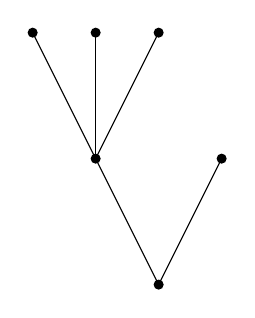
\begin{tikzpicture}[scale=.8]
%\draw (-1,-2) grid (5,2);
\filldraw[black] (0,0) circle (2pt);
\filldraw[black] (1,2) circle (2pt);
\filldraw[black] (-1,2) circle (2pt);
\filldraw[black] (-2,4) circle (2pt);
\filldraw[black] (-1,4) circle (2pt);
\filldraw[black] (0,4) circle (2pt);
\draw (0,0) -- (1,2);
\draw (0,0) -- (-1,2);
\draw (-1,2) -- (-2,4);
\draw (-1,2) -- (-1,4);
\draw (-1,2) -- (0,4);
\end{tikzpicture}


\section{Denbora birparametrizazioa.}


\subsection{Denbora birparametrizazioa.}

Demagun jatorrizko ekuazio diferentziala,

\begin{equation*}
\dot{y}=f(y(t)),
\end{equation*}

non $y$ menpeko aldagaia eta $t$ aldagai askea den.

\paragraph*{} Aldagai askeari aldaketa bat aplikatuz ($s()$ izeneko funtzio), ekuazio diferentziala leuntzea lortuko dugu. 

\begin{equation*}
y=z,
\end{equation*}

\begin{equation*}
\frac{dt}{d\tau}=s(z)
\end{equation*}

\paragraph*{} Honako garapena egingo dugu aldagai berriarekiko ($\tau$) ekuazioak lortzeko.

\begin{equation*}
y=z \ \ \Rightarrow \ \ \frac{dy}{dt}=\frac{dz}{d \tau} \ \frac{d \tau}{dt} \ \Rightarrow \ \frac{dz}{d \tau}= s(z) \ f(y(t)) 
\end{equation*}

\paragraph*{} Sistema berrian, mugimendua $z(\tau)$ funtzioak deskribatzen du: $z$ aldagai berria $\tau$ aldagai askearen menpekoa da. 

\subsection{Adibidea.}

Esperimentu honetan, IRK metodoan denbora birparametrizazioa modu errezean aplika daitekeela erakutsi nahi dugu. N9-Body probleman, merkurio ezentrizitate handiena duen planeta da: merkurio araberako denbora birparametrizazioa planteatuko dugu.

\begin{equation}
s(q)=r_{10}^{3/2}
\end{equation}

\begin{equation}
r_{10}=\|q1-q0\|_2
\end{equation}

non $q_1=(q1_{x},q1_{y},q1_{z})$ merkurio plantearen kokapena eta $q_0=(q0_{x},q0_{y},q0_{z})$ eguzkiaren kokapena den.

\section{Laburpena.}